\documentclass[12pt]{article}
\usepackage{amsmath}
\usepackage{graphicx}
\usepackage{listings}
\usepackage{verbatim}
\def\pp{\par\noindent}
\newcommand{\problem}[1]{\bigskip\pp\textbf{Part #1}\smallskip}
\renewcommand{\part}[1]{\smallskip\pp\textbf{#1)}\indent}
\newcommand{\given}{$\vert$~}
\newcommand{\prob}{\text{Pr}}
\begin{document}
\lstset{basicstyle=\small,language=Python,tabsize=2}
\centerline{CSE 544 - Final Project}
\centerline{Andrew Burford 112251367}
\centerline{Daniel Billmann 114715276}
\centerline{Efthimios Vlahos 110540896}

\problem{1}
\par We used pandas to read in the csv data and store it in a pandas
DataFrame object. Data was cleaned independently for each column of
data we are interested in. i.e. the daily cases in a specific state
was cleaned separately from the daily cases in a different state.
There were no empty rows within the CSV data we had to worry about.
While decumulatizing the rows, we noticed an issue in the cumulative
deaths data within MA.
\pp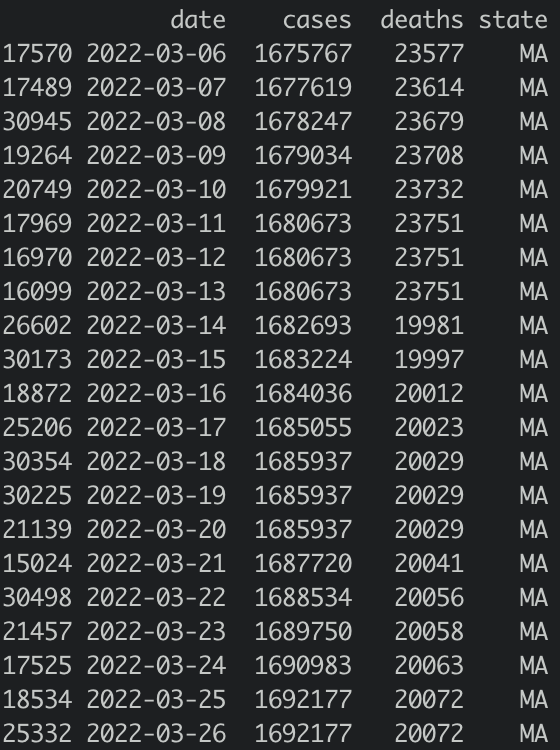
\includegraphics[scale=0.5]{cumulative_error.png}
\par You can see that on March 14th, 2022, the cumulative total drops.
This results in a negative number of deaths for this day, but it ends
up not mattering because this data point is dropped after applying
Tukey's rule. Here is the output of our cleaning script:
\verbatiminput{cleaning.log}

\problem{2}
\part{a}
\verbatiminput{part_a.log}
\part{b}
\verbatiminput{part_b.log}
\part{c}
\verbatiminput{part_c.log}
\pp\includegraphics[scale=1]{2c.pdf}
\part{d}
\verbatiminput{part_d.log}
\part{e}
\verbatiminput{part_e.log}

%\problem{1}
%\part{a} 
%\pp\includegraphics[scale=0.2]{1a}
%\begin{lstlisting}
%\end{lstlisting}

\end{document}
% vim:textwidth=70
